\section{Make people aware of how much money, time, climate they are using on commuting}
\label{sec:make-people-aware-of-how-much-money-time-climate-they-are-using-on-commuting}

Commuting is a part of our everyday life and especially of people in employment.
A study from Denmark’s statistic clearly shows that out of around three million people only 185 thousand people doesn't
commute to work.
This means \(83.65\,\%\) commute to work in Denmark~\cite{erhvervspendling2021}.
% TODO Reference figure in a more meaningful way.
See~\ref{fig:figure} for more information.

As we mentioned earlier people are uninformed about how much emissions they are using while choosing their desired
commuting option.
The desired preference of the commuting can change the way people commutes.
A study made in 2021 on commuting showed which transport option users would pick depending on what their preferences
were.
Here we can clearly see that public transport is preferred when the priority is saving time, cost or being
environmentally friendly while walking or cycling were more preferred when health was the priority.
This is interesting because if people had the opportunity to select either economy, time or sustainability as a
preference when commuting they could use alternative transport options.
Furthermore, this could possibly promote sustainable commuting.
This may be important as sustainable living is becoming more trending than ever.
This is a direct result of people becoming more aware of how their choices can have an effect on the environment they
live in~\cite{spark2023}.
Research done by Capgemini research shows a sturdy connection between sustainability and significant business benefits.
This means that customer loyalty and revenue increases by having a focus on being sustainable~\cite{capgemini2020}.
The enlarged focus on sustainability is because the future shoppers are the new youth, and they prioritize
sustainability more than millennials.
This shows that it could be environmentally beneficial if the people had a saying in how they prefer to commute.

Commuting can also influence mental health and well-being as it can cause an increase in stress level.
This is apparent in some research.
One suggests that one of the factors is that the commuters have a difficulty in appreciating their way of commuting.
The author furthermore explains that the governments must prioritize what the commuters prefer.
Beside these workers can have an incline in stress levels as they have deadlines and specific meeting times.
By this we can derive that having the opportunity to travel to your destination fastest as possible can be beneficial
for the health~\cite{koslowsky2013}.
Another research made a study on 208 people who were rail commuters In New York and made an interesting discovery.
It showed that the longer time that they commuted the more their cortisol level increased.
This means that time duration of commuting is an important factor.
Therefore, it is essential that people commuting can have an influence on time spent commuting.
Another critical aspect is how commuting effect the economy of people.
Research shows that the average American citizen spends \SI{8466}[\$]{} on co commute expenses.
There is different cost involved depending on which transport options you use.
For example, \(76\,\%\) of commuters use their personal vehicle.
They have some extra expenses besides buying a car.
The average driver spends \SI{1771}[\$]{} on full car insurance and furthermore they spend money on car maintenance
and occasionally after 5000 miles they need to get their vehicles' oil changed.
This could be a challenge as research shows that 1 out of 3 drivers can't afford sudden unexpected car repairs.
The study suggests that using public transport, bike or scooter to work will cost less.
This change could be difficult as commuting in a personal vehicle could be much more time efficient~\cite{bankrate2023}.
A study showed that the working poor who commuted by public transport spend \(10\,\%\) of their income on commuting
compared to \(21\,\%\) when commuting in their car.
The working poor prefer saving money because this means they can spend a larger portion of their income on other
expenses like food, healthcare, household supplies and saving for the future.
From this, it is apparent that especially the poorer people could have an advantage by having the opportunity to
commute by their preferences.
This could improve their economy as the working poor tend to use the least expensive options of commuting, like
carpooling, van pooling, biking, walking and public transport.
Comparing this to people with higher income they are more inclined to spend more on commuting~\cite{bankrate2023}.
% TODO Reference figure in a more meaningful way.
See~\ref{fig:figure2} for more information.

\begin{figure}
    \centering
    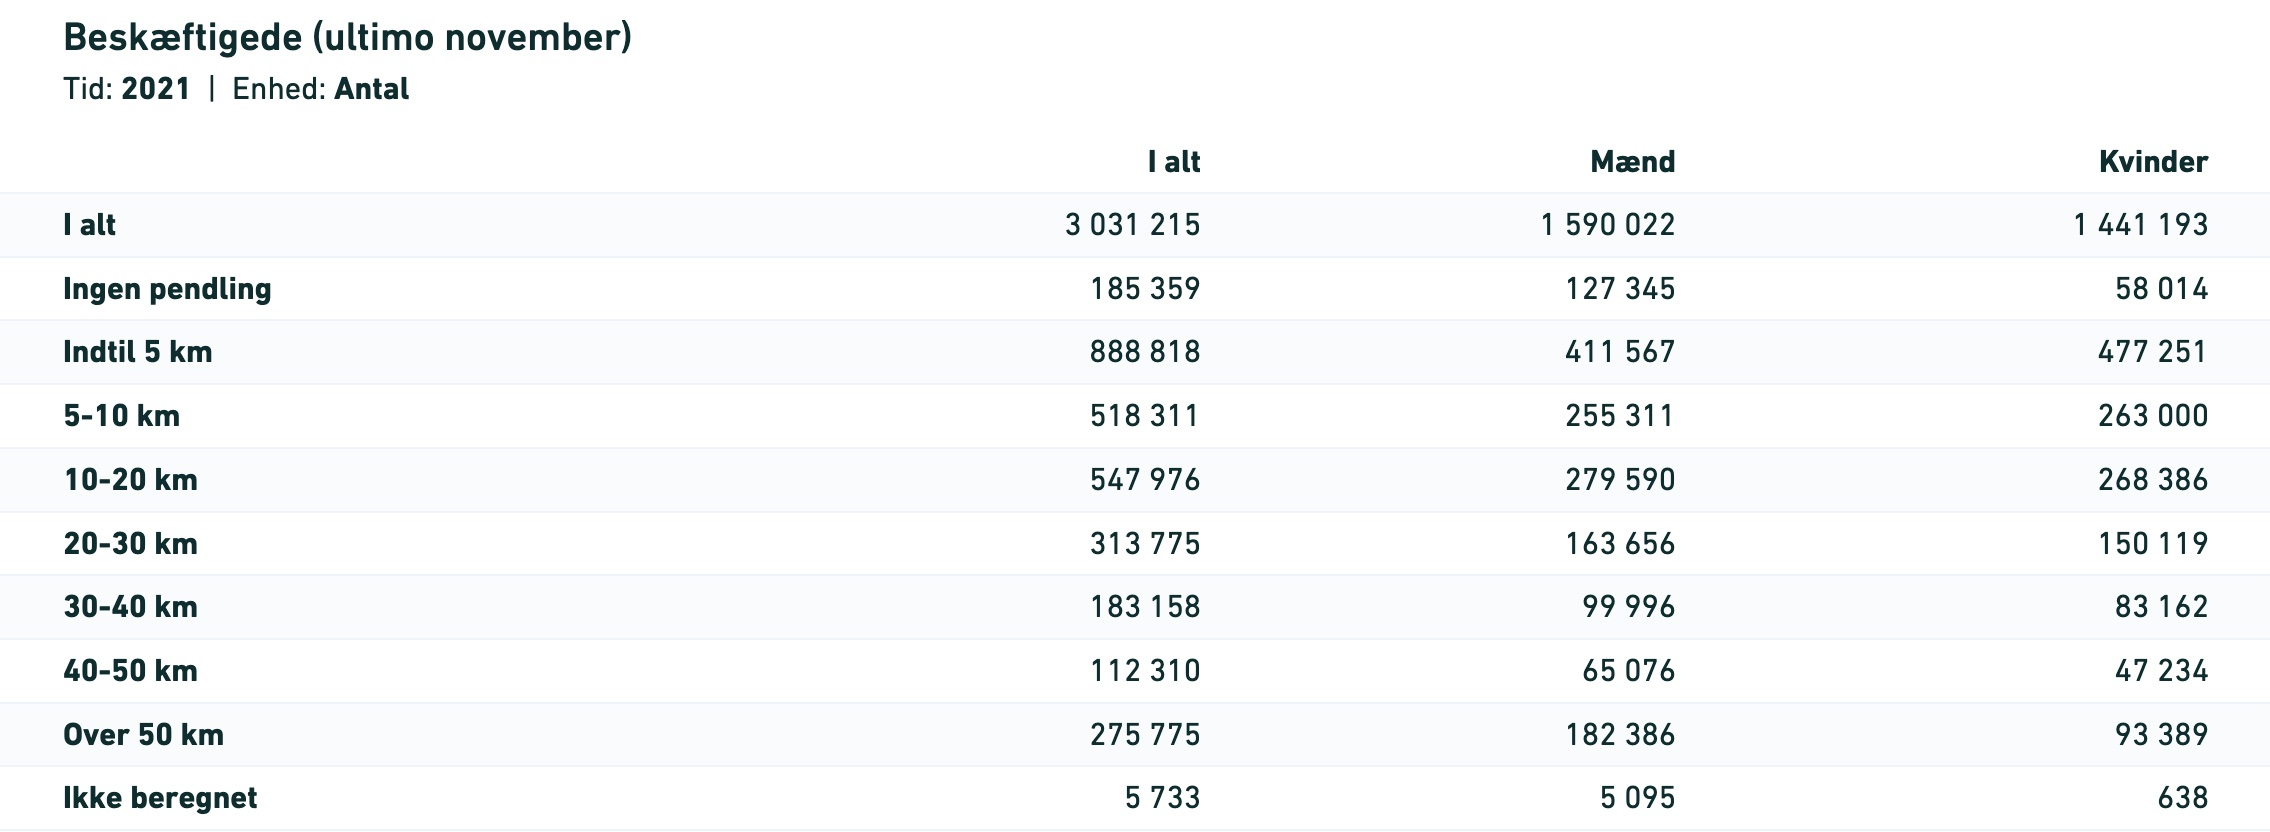
\includegraphics[width=\textwidth]{images/stats}
    \caption{A picture of a gull.}
    \label{fig:figure}
\end{figure}

\begin{figure}
    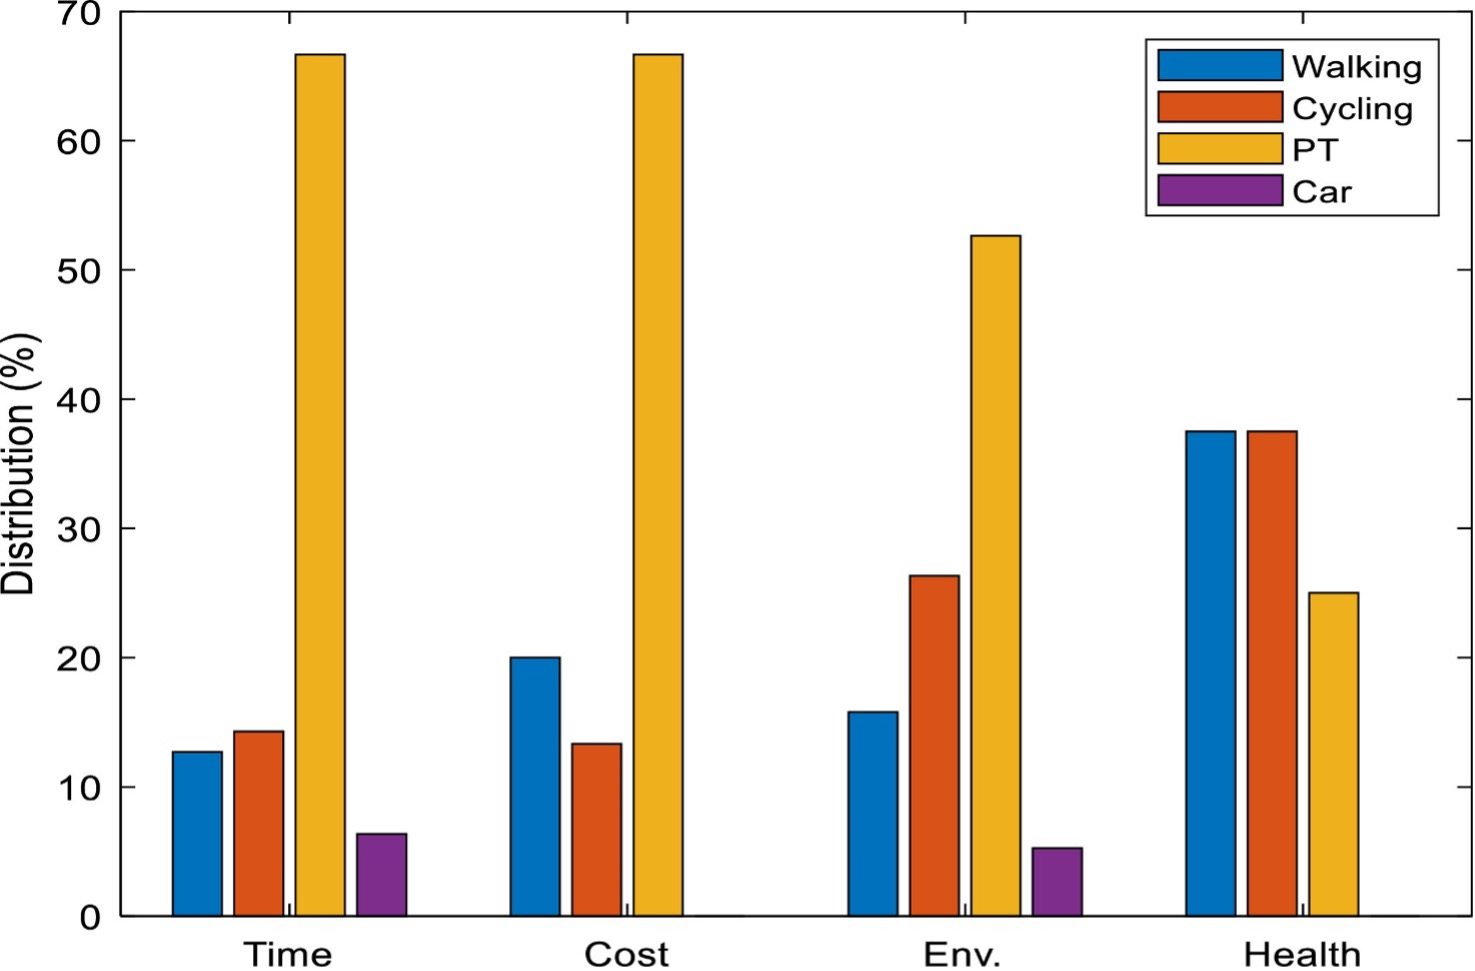
\includegraphics[width=\textwidth]{images/stats-2}
    \caption{A picture of a gull.}
    \label{fig:figure2}
\end{figure}
